\section{Results}
\label{sec:results}

Here, we will present the main results which is the performance of both PCA and GPR as foreground removal methods. First, the results for PCA will be presented, secondly, GPR.

\subsection{Principal Component Analysis}

The performance of the PCA foreground removal was evaluated by comparing the recovered residual signal to the true cosmological signal through the cylindrical and spherically averaged 1D power spectra. First, we will discuss the choice of foreground principal components. Then, the results from the foreground removal which is the 1D and cylindrical power spectrum will be discussed. Finally, we will finish with a review on the overall performance of PCA.

\subsubsection{Foreground Principal Components}

The choice of $N_{FG} = 3$ was decided on based by inspection of the eigenvectors and eigenvalues. This choice of $N_{FG}$ components has a trade-off where too few components leave residual foreground, while too many mean the HI signal might be subtracted. The first three modes captured the foreground-dominated variance while the remaining modes were consistent with the cosmological signal. 

% [1] https://arxiv.org/pdf/2105.12665
The choice of $N_{FG} = 3$ is much lower than what was used in [1] which used $N_{FG} = 6$ and $N_{FG} = 7$. This is likely due to their more complex data and our data only consisting of the cosmological signal and the foreground. The results suggests that three components is a reasonable choice for this simulation, though a more rigorous approach could be taken which involves cross-validating the choice of $N_{FG}$ against the recovered power spectrum as a function of component number. 

\subsubsection{Cylindrical Power Spectrum}

The cylindrical power spectrum of the true HI power spectrum, the residual signal after PCA cleaning, and their ratio (see \Cref{fig:cylindrical_power_spectrum_None_None}) was used as an assessment of the foreground cleaning. The ratio panel provided the clearest diagnostic of the cleaning performance. At high $k_{\parallel}$, the ratio is close to unity and uniformly red, indicating that the recovered signal is in good agreement with the true HI power spectrum in these modes. This is physically expected as high $k_{\parallel}$ modes correspond to small-scale structure along the line of sight that varies rapidly with frequency and is therefore largely orthogonal to the spectrally smooth foreground components removed by PCA. 

% [1] https://academic.oup.com/mnras/article/446/4/3545/2891891
% [2] https://iopscience.iop.org/article/10.1086/668105/pdf#:~:text=This%20work%20was%20originally%20developed%20for%20PCA,underlying%20methodology%20is%20specific%20to%20astronomical%20spectra.
% [3] http://academic.oup.com/mnras/article/478/3/3640/4995230#118057951
% [4] https://arxiv.org/pdf/2407.21626
However, at low $k_{\parallel}$, the ratio drops below unity, indicating significant signal loss. Here, the 21\,cm signal shares spectral structure with the foregrounds and cannot be cleanly separated by PCA. This inevitably removes some genuine HI signal alongside the foreground components, a known limitation of blind component separation techniques [1] [2]. This signal loss at low $k_{\parallel}$ is consistent with findings in [3] and [4], who report the same characteristic suppression of modes at low $k_{\parallel}$ from PCA cleaning. 

Through inspection of the ratio panel, a minimum threshold of $k_\parallel = 0.4$\,Mpc$^{-1}$ was defined and the foreground cleaning of the signal was redone excluding modes below these values. Minimum thresholds with values below this were found to still show cosmological signal loss. While minimum threshold with values larger than this were found to as well closely match the true HI signal, the goal was to find the smallest threshold which maximised foreground cleaning and minimised cosmological signal loss. 

\subsubsection{1D Power Spectrum}

\begin{figure}[t!]
    \centering
    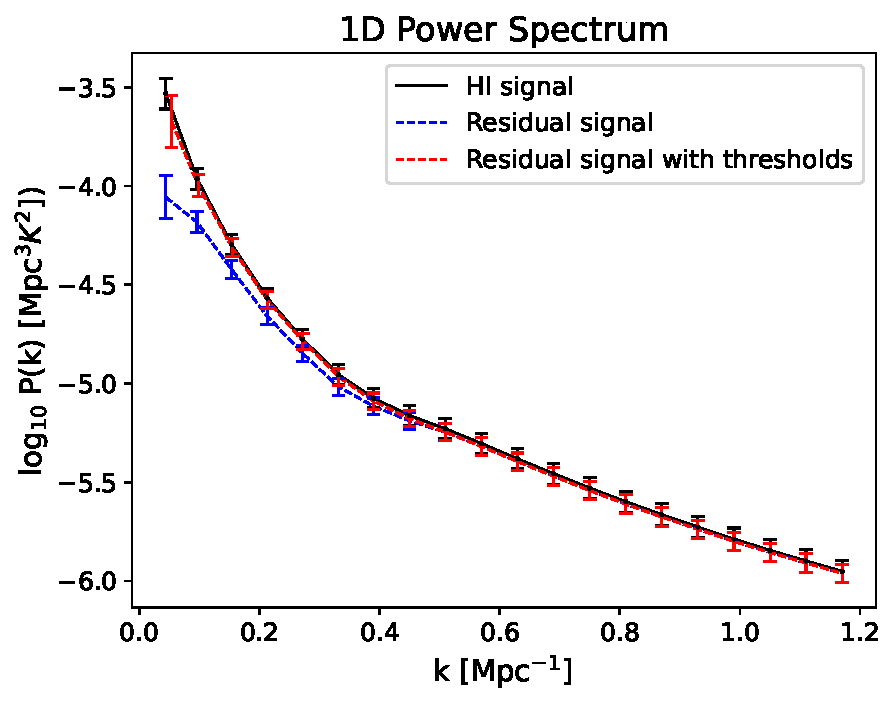
\includegraphics[width=1\linewidth]{outputs/week9/1d_log_power_spectrum_[0, 0.04]_None_both.pdf}
    \caption{The logarithmic spherically averaged 1D power spectrum from of the HI signal with no foreground removal (black), and the residual signal after PCA foreground removal without any minimum thresholds applied (blue) and the residual signal after PCA foreground removal with minimum thresholds of $k_\parallel = 0.4$\,Mpc$^{-1}$ (red). This was run for 100 realisations with the mean used as the datapoints and the standard deviation used as the error bars.}
    \label{fig:1d_log_power_spectrum_0_0.04_None_both}
\end{figure}

The spherically averaged 1D power spectrum with the true HI signal and the residual signal before and after applying the minimum $k$ thresholds can be seen in \Cref{fig:1d_log_power_spectrum_0_0.04_None_both}. Since foreground cleaning was run with 100 independent realisations from 100 fixed seeds, this allowed for uncertainties to be quantified for both the residual signal and the cosmological HI signal, taking into account not only the foreground cleaning but also cosmic variance. Thus, error bars are also seen on the HI signal. 



Prior to applying the minimum thresholds, the residual signal (shown by the blue line) follows the true HI signal (shown by the black line) at large $k$ but shows a clear deviation at low $k$, consistent with the signal loss identified in the cylindrical power spectrum ratio panel due to some of the genuine cosmological signal being removed with the foreground components.

After applying the minimum thresholds of and $k_\parallel = 0.4$\,Mpc$^{-1}$, the residual signal (shown by the red line) shows a stronger agreement with the 21\,cm signal across the whole $k$ range, with the curve lying within 1$\sigma$ of the HI signal error bars across the whole $k$ range. We can see that the error bars are uniform in size at large $k$ but towards lower $k$ the error bars for the residual signals grow larger, especially for the residual signal with the minimum thresholds. This is expected and represents the increased variance in the residual signal as a result from the cleaning. 

It is also important to note that the residual signal with thresholds does not extend all the way to $k = 0$\,Mpc$^{-1}$ and this is a consequence of excluding these minimum thresholds as these datapoints are completely excluded from the analysis. So, while this signal does recover the true HI signal well, there is genuine cosmological signal loss. 

\subsubsection{Overall Performance}

Overall, the PCA foreground removal performs well within the defined k-thresholds, recovering the HI power spectrum well throughout the whole $k$ range. The primary limitation is the signal loss at low $k_{\parallel}$, which is a consequence of the assumption that the foregrounds occupy lower values of $k$. This assumption breaks down when the HI signal has correlated structure on scales comparable to the foreground lengthscale and can be seen here where parts of the cosmological signal is also removed. 

This analysis would be much more difficult is a more realistic dataset were used or if a more realistic foreground model were used. The foreground signal used in this analysis assumes a single spectral index across the sky, whereas real foregrounds have spatially varying indices which would make PCA separation more difficult.

% [1] https://iopscience.iop.org/article/10.1088/2041-8205/763/1/L20
% [2] https://iopscience.iop.org/article/10.1088/0004-637X/815/1/51
In the case of more complex data with components more representative of true observations, another method which could be considered instead of applying minimum $k$ thresholds to mitigates signal loss is to use a transfer function [1], [2]. Instead of excluding the modes which cause the most signal loss, a transfer function is able to keep all $k$ modes but corrects for the signal loss at each one. Instead of completely removing low $k$ modes, it attempts to boost them by the expected suppression factor. However, while this preserves cosmological information, a limitation is that it amplifies noise and foreground residuals while the signal is being boosted. Given the significant foreground residuals present at low $k_{\parallel}$ in this analysis, applying a transfer function correction would amplify both the HI signal and the residual foreground contamination simultaneously, making the k-threshold approach the more conservative and appropriate choice here.

%Additionally, this analysis only used a small range of frequencies whereas other analysis' use a broader range. While this simplifies the foreground cleaning, this smaller range allowed for 100 realisation to be run, allowing for the foreground cleaning and cosmic variance to be taken into consideration and error bars to be quantified and plotted on the power spectra, whereas other simulation studies have a larger frequency range but only show a single realisation.

\subsection{Gaussian Process Regression}

\begin{figure*}[h!]
    \centering
    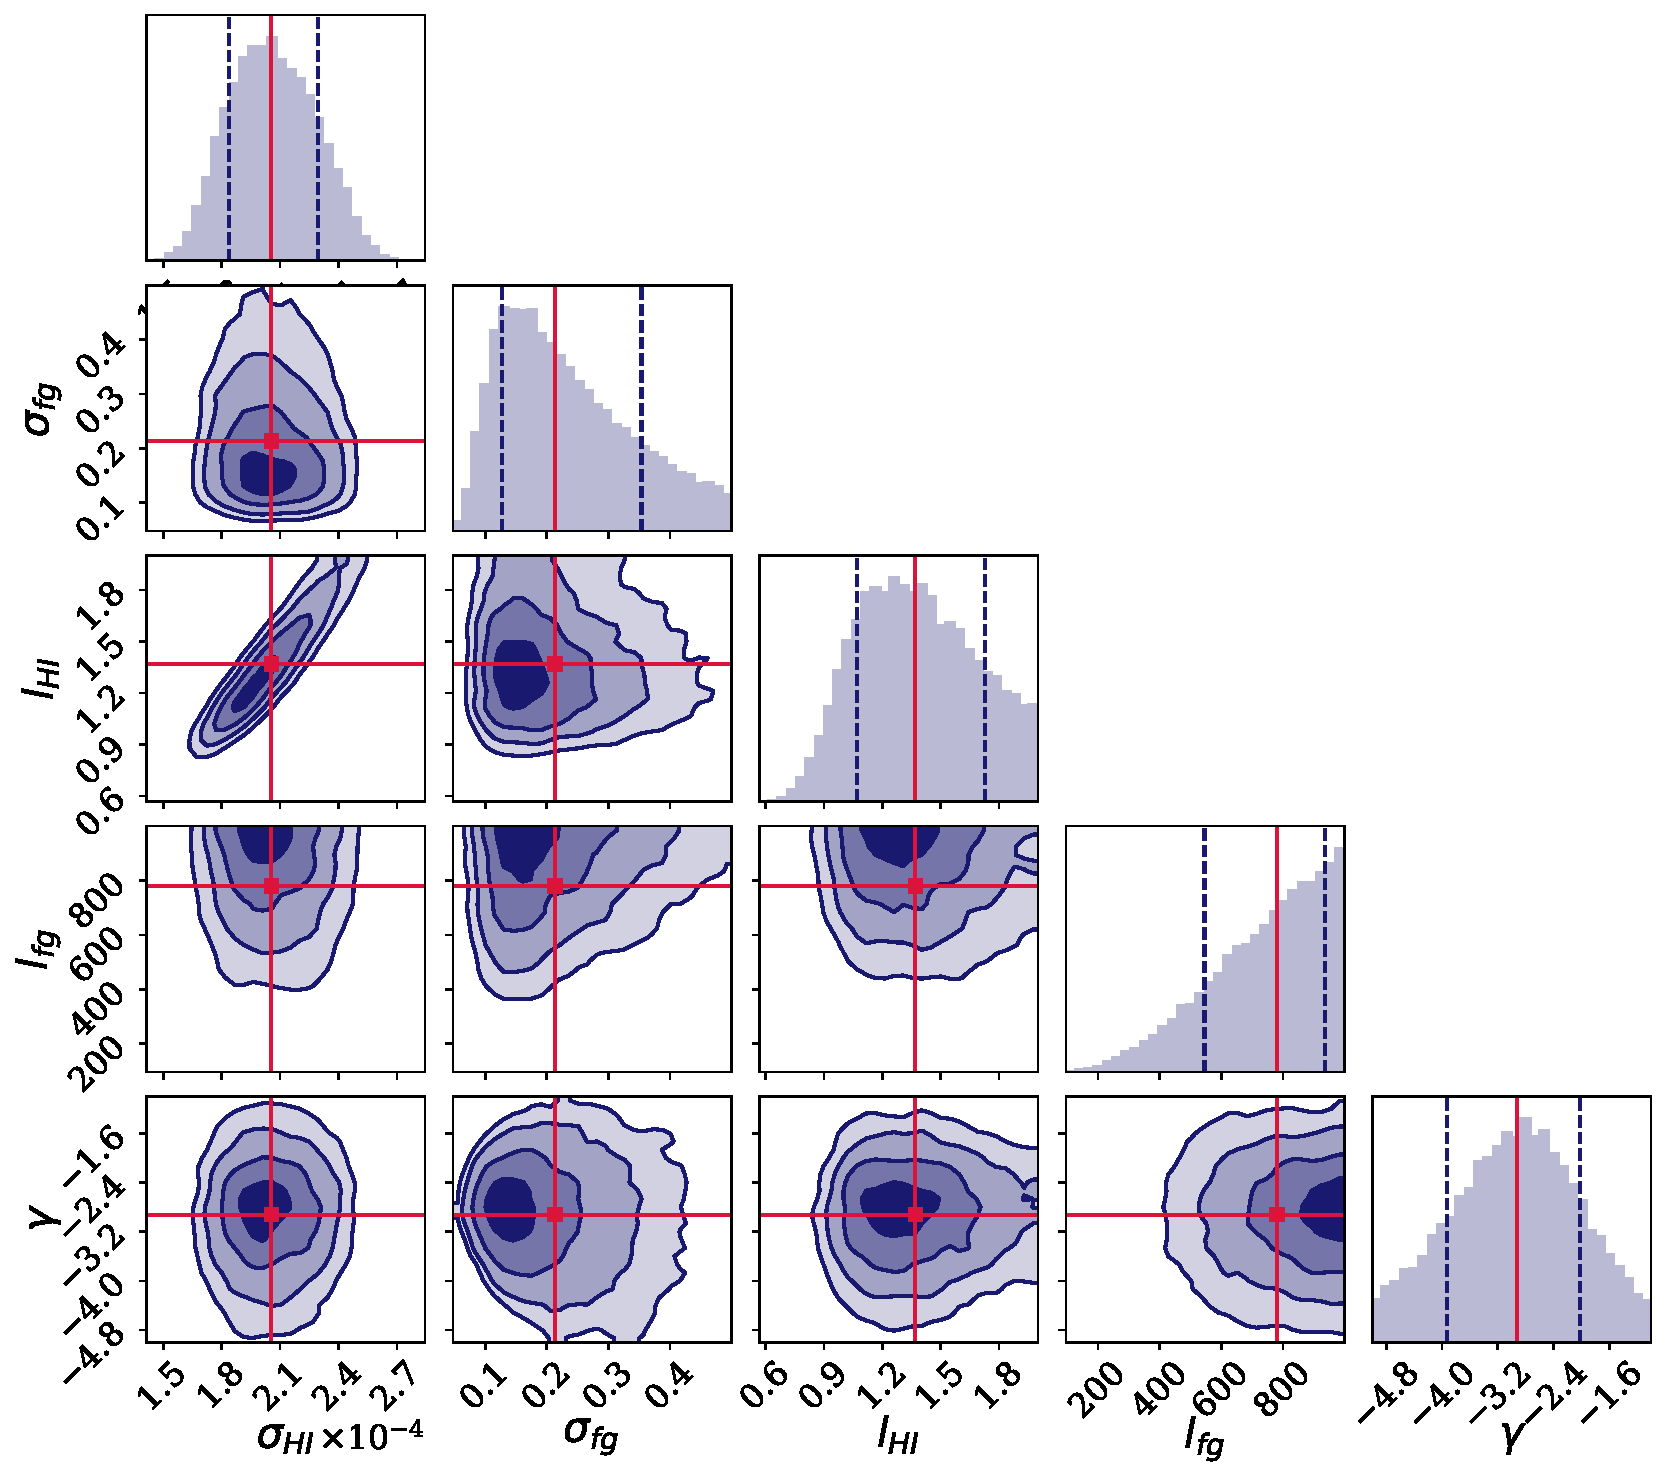
\includegraphics[width=0.71\linewidth]{outputs/week8/final_corner_plot_values.pdf}
    \caption{Posterior distribution for the MCMC sampling from GPR foreground cleaning using the exponential kernel to model the 21\,cm cosmological signal and the spectral index modified RBF kernel to model the foreground. The panels show the 1D marginals and the 2D joint constraints. The contours corresponds to the 1, 2, and 3$\sigma$ credible regions.}
    \label{fig:final_corner_plot_values}
\end{figure*}

\begin{figure*}[h!]
    \centering
    \includegraphics[width=0.71\linewidth]{outputs/week8/mcmc_chain_with_sp_indx_fg_no_noise.pdf}
    \caption{Trace plots for the MCMC sampling from GPR foreground cleaning using the exponential kernel to model the 21\,cm cosmological signal and the spectral index modified RBF kernel to model the foreground.}
    \label{fig:mcmc_chain_with_sp_indx_fg_no_noise}
\end{figure*}

Here, we will discuss the results of foreground removal using GPR. Different combinations of the kernels functions, with different initial guesses, bounds, and optimisation algorithms were tested and their LMLs compared to find the one which fit the data the best. The optimisation algorithm which found to provide the best results within the minimise function from the optimise module of SciPy was the Nelder-Mead algorithm.

The exponential function (\Cref{eq:exp}) was found to fit the 21\,cm signal the best in all cases. Additionally, the spectral index modified RBF kernel (\Cref{eq:RBF_sp_indx}) performed the best in comparison to the normal RBF kernel (\Cref{eq:RBF}), as expected as it better models the smooth foregrounds (see \Cref{fig:rbf_kernel_w_sp_indx_vs_foreground_covariance}). It was this kernel combination which gave the highest Bayes Factor and was used for MCMC Sampling.

First, we will go over the hyperparameter estimations that came as a result of the MCMC Sampling  using the kernel combination described above along with the MCMC parameter convergence. Then, we will discuss the results from the foreground removal which is the 1D and cylindrical power spectrum. Finally, we will finish with a review on the overall performance of GPR.

\subsubsection{Hyperparameter Estimation}

\begin{table*}[bt!]
    \centering
    \renewcommand{\arraystretch}{2}
    \caption{Median and $1\sigma$ estimates for the hyperparameters.}
    \label{tab:hyperparameters}
    \begin{tabular}{|l|ccccc|}
        \hline
        Hyperparameter & $\sigma_{HI}$ [mK$^2$] & $\sigma_{fg}$ [mK$^2$] & $l_{HI}$ [MHz] & ${l_{fg}}$ [MHz] & $\gamma$ \\
        \hline
         & 2.05 $^{+0.24}_{-0.22}\times10^{-4}$ & 0.21 $^{+0.14}_{-0.09}$ & 1.37 $^{+0.36}_{-0.30}$ & 780.37 $^{+156.62}_{-234.79}$ & -2.92 $^{+0.91}_{-1.01}$ \\
         \hline
         \hline
        Prior & $\mathcal{U}$ (1 $\times 10^{-6}$, 0.5)& $\mathcal{U}$ (1$\times 10^{-6}$, 0.5) & $\mathcal{U}$ (0.01, 2.0) & $\mathcal{U}$ (10.0, 1000.0) & $\mathcal{U}$ (-5.0, -1.0) \\
        \hline
    \end{tabular}
\end{table*}

\begin{figure*}[t!]
    \centering
    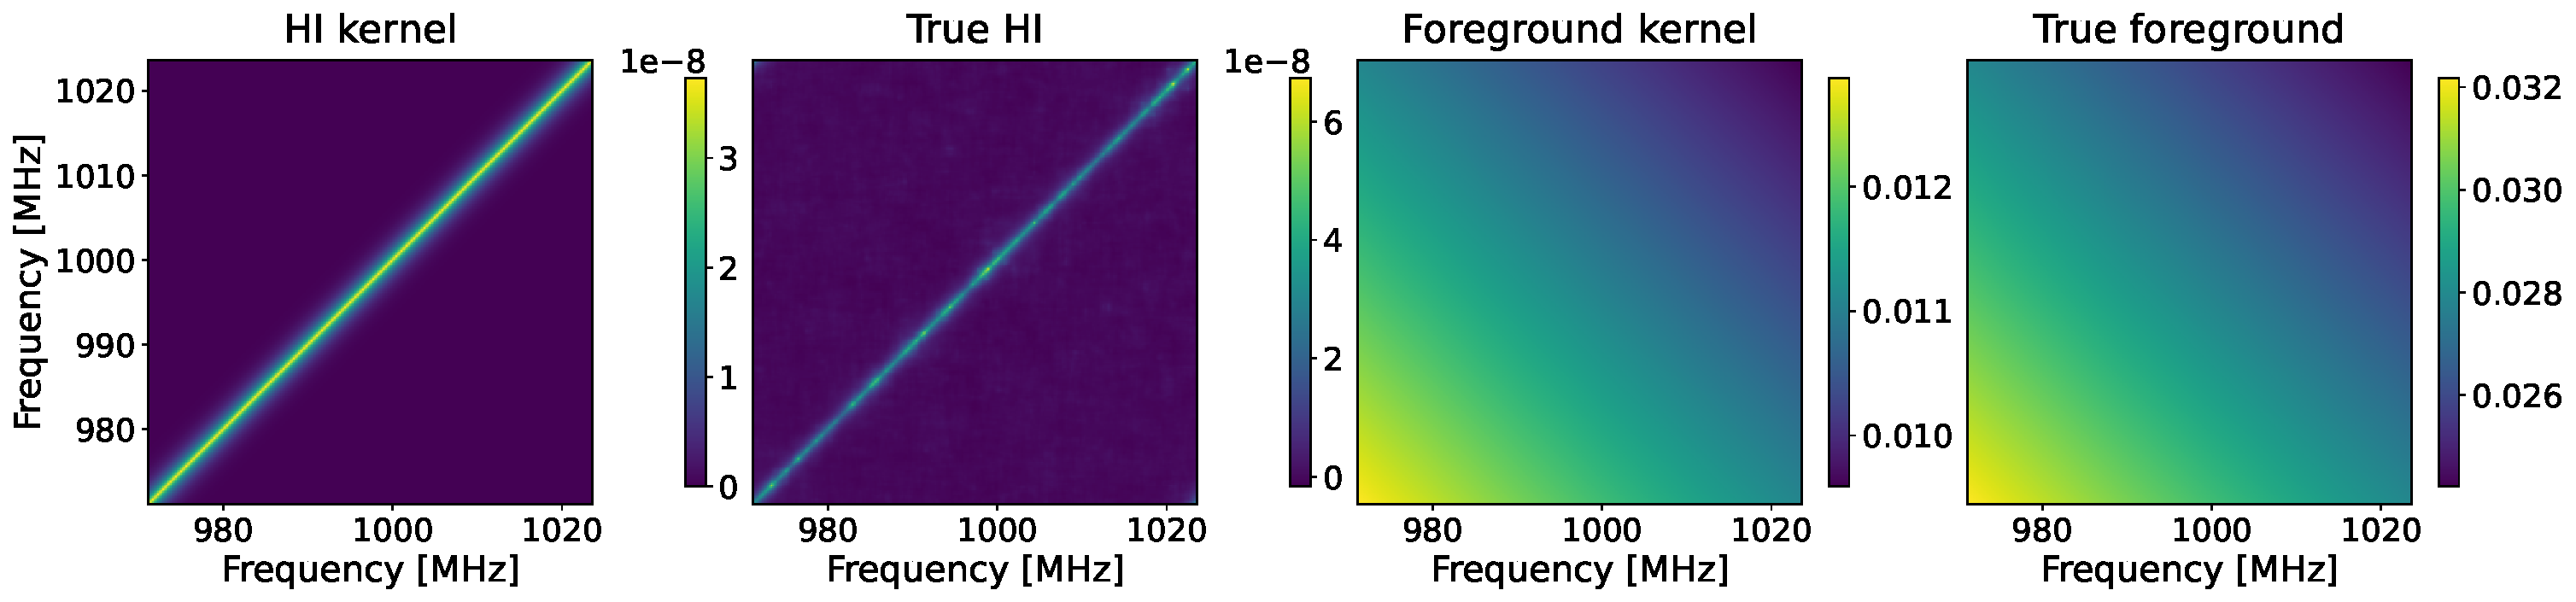
\includegraphics[width=1\linewidth]{outputs/week8/kernel_comparison_mcmc_with_sp_indx_no_noise.pdf}
    \caption{Comparison of the fitted GPR kernels against the true component covariances. From left to right: the fitted HI kernel (exponential), the true HI covariance, the fitted HI kernel (spectral-index-modified RBF), and the true foreground covariance.}
    \label{fig:kernel_comparison_mcmc_with_sp_indx_no_noise}
\end{figure*}

The posterior distributions of the GPR hyperparameters were explored using MCMC sampling, with the resulting corner plot shown in \Cref{fig:final_corner_plot_values}. The model includes five hyperparameters: the amplitude and the length scale of the HI signal kernel and the foreground kernel ($\sigma_{HI}$, $\sigma_{fg}$, ${l_{HI}}$, ${l_{fg}}$), and the foreground spectral index ($\gamma$). All together, these parameters control how the GPR model separates the spectrally smooth foreground from the HI signal which varies rapidly with frequency. A summary of the recovered hyperparameter values can be seen in \Cref{tab:hyperparameters}. 

The HI amplitude $\sigma_{HI}$ recovered is the most tightly constrained out of all the hyperparameters and suggests that the GPR model is correctly identifying the amplitude of the HI fluctuations even in the presence of foreground contamination. In each combination of the different kernel optimisations run before the MCMC sampler, $\sigma_{HI}$ was the most consistently recovered each time.

The recovered HI lengthscale $l_{HI}$ is moderately constrained. While this posterior peaks, it also has a tail towards larger values which is not as expected. Since this parameter controls how smooth the signal is across frequency and a smaller value results in more rapid variations, this is not consistent with the HI signal. It is interesting to see the extremely diagonal covariance plot between $\sigma_{HI}$ and $l_{HI}$, which is a contrast to all the other covariance plots, highlighting these two parameters are highly correlated.

On the other hand, the foreground amplitude $\sigma_{fg}$is considerably less well constrained. This broad and asymmetric posterior reflects a degeneracy in foreground modelling where the total foreground component can be reproduced by different combinations of amplitude and correlation length. This means that it is difficult to confine these parameters independently.

The foreground lengthscale $l_{fg}$ recovered has a particularly large and asymmetric uncertainty. The posterior rises steeply and has a long tail towards higher values, suggesting the data is consistent with a wide range of $l_{fg}$. This is an issue which kept on arising upon trying different optimisation methods. No matter what initial guesses or range of bounds were used, $l_{fg}$ would consistently hit the upper bound of the range every time, even if the bound was made smaller or wider. Physically, this large $l_{fg}$ corresponds to foreground emissions that is highly correlated in frequency and therefore very smooth which is consistent with what we expect with synchrotron-dominated foregrounds. However, the poor constraint indicates that the frequency range used may be insufficient to fully characterise $l_{fg}$. A wider bandwidth may be beneficial for this hyperparameter.

Finally, the foreground spectral index $\gamma$ is recovered with a broad posterior and the injected true value of -2.7 being within the uncertainties. While this median value is consistent with the expected behaviour, the wide posterior reflects the difficulty of constraining the spectral shape which is possibly due to the relatively narrow frequency range. The diffuse joint posterior for $l_{fg}$ and $\gamma$ in the corner plot suggests that the data cannot distinguish between the different combinations of these hyperparameters. This physically makes sense as a steeper $\gamma$ and a longer $l_{fg}$ can produce similar foreground covariance structures, resulting in these hyperparameters being difficult to constrain independently.

The MCMC trace plots for all five hyperparameters are shown in \Cref{fig:mcmc_chain_with_sp_indx_fg_no_noise}. Trace plots are important in MCMC as they verify that the chains have converged and they explore the parameter space efficiently. Each coloured line represents an individual walker's trajectory through parameter space over 10,000 steps. For a well-converged sampler where the walkers efficiently explore the posterior distribution, the traces should be dense bands that are stationary, meaning the chain has converged around a mean with variance variance with no upward or downward trends. 

For all hyperparameters, the plots demonstrate good mixing across all walkers. The mean acceptance fraction for the burn-in and sampling were both approximately 0.46 which shows there was an optimal balance between step size and efficient exploration of the posterior. $\sigma_{HI}$ is the most well well converged and stable, consistent with the constrained posteriors seen in the corner plot. However, $l_{HI}$, $\sigma_{fg}$, $l_{fg}$, and $\gamma$ show the walkers explore a wide range of values throughout the run, often hitting the lower and upper bounds throughout the run. While these chains do not show any systematic drift and appear stationary, this large spread is consistent with the broad, poorly constrained posteriors seen in the corner plot. This confirms the degeneracies the foreground model posses and that the difficulty in constraining these hyperparameters is a feature of the posterior landscape rather than the sampler failing to converge. The fitted kernels, along with the true covariance signals, can be seen in \Cref{fig:kernel_comparison_mcmc_with_sp_indx_no_noise}.

\subsubsection{Cylindrical Power Spectra}

\begin{figure*}[t!]
    \centering
    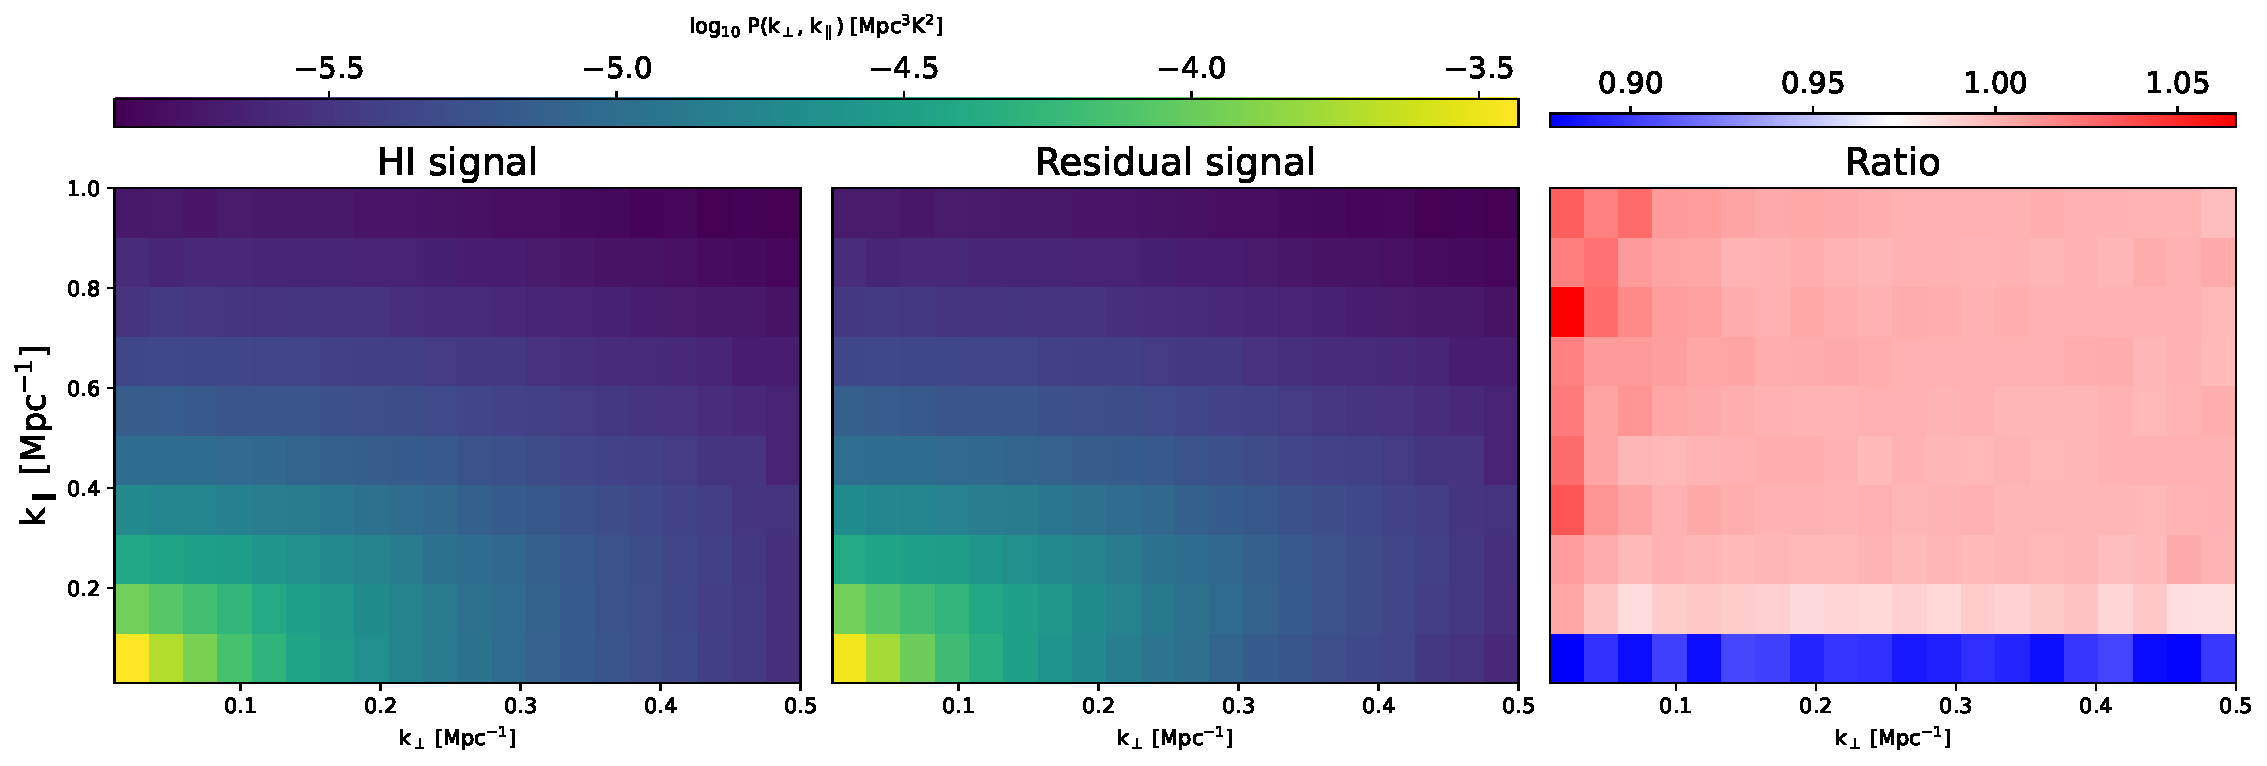
\includegraphics[width=1\linewidth]{outputs/week9/gpr_cylindrical_scipy_with_no_noise_and_sp_indx.pdf}
    \caption{The cylindrical power spectra for the GPR foreground cleaning method, with the HI signal, the residual total signal (HI signal and foreground) after foreground removal, and the ratio between residual and the HI signal, from left to right.}
    \label{fig:gpr_cylindrical_scipy_with_no_noise_and_sp_indx}
\end{figure*}

\begin{figure}
    \centering
    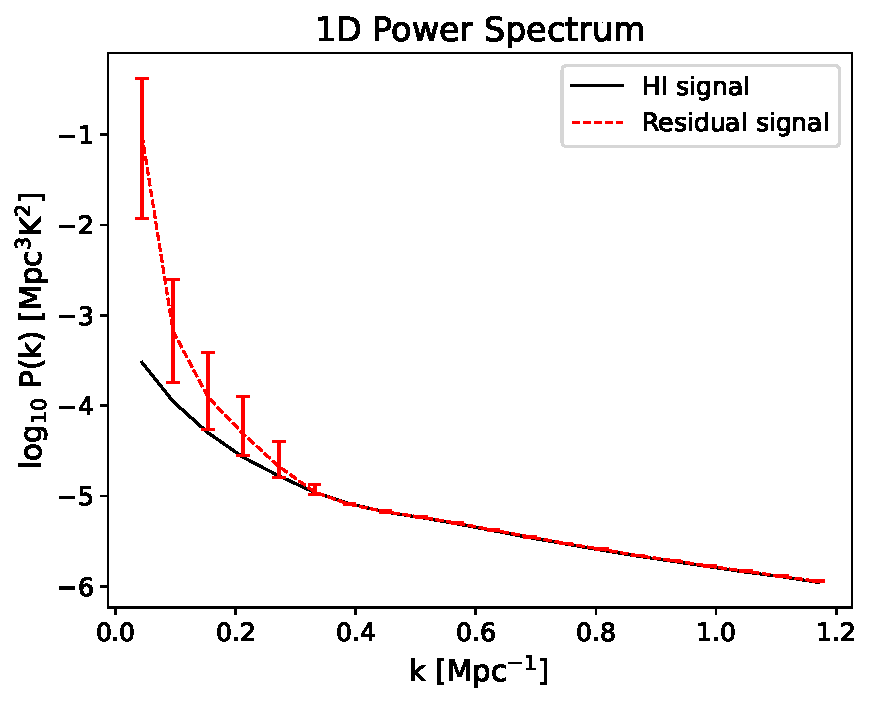
\includegraphics[width=1\linewidth]{outputs/week9/final_power_spectrum_1.pdf}
    \caption{The logarithmic spherically averaged 1D power spectrum from of the HI signal with no foreground removal (black), and the residual signal after GPR foreground removal (red). This was run for 1,000 realisation from the MCMC samples, where the datapoints are the median values and the 16th and 84th percentiles were used as the error bars for the residual signal.}
    \label{fig:final_power_spectrum_1}
\end{figure}

The cylindrical power spectrum provides some more information on the foreground removal by separating modes along the line of sight ($k_{\parallel}$) from transverse modes ($k_{\perp}$). \Cref{fig:gpr_cylindrical_scipy_with_no_noise_and_sp_indx} shows the true HI power spectrum, the residual signal from the GPR clean, and their ratio. 

The ratio panel is the clearest diagnostic on the success of the foreground cleaning. We can see that throughout the panel, the ratio is close to unity while at low $k_{\parallel}$ and high $k_{\perp}$, at the smaller spatial scale, there is cosmological signal loss. Additionally, there are $k$ modes at low $k_{\perp}$, suggesting under-cleaning of the large spatial scale. 

\subsubsection{1D Power Spectrum}

The spherically averaged log 1D power spectrum before and after GPR foreground removal is shown in \Cref{fig:final_power_spectrum_1}. The black curve represents the true HI power spectrum whereas the red dashed curve shows the recovered power spectrum after GPR cleaning.

At high $k$ values, the residual power spectrum lies exactly on the true HI signal, showing a perfect recovery. However, at lower $k$, which refers to large scales, values the signal deviates largely from the true signal. This is consistent with the fact that foregrounds are most dominant at low frequencies and so there is some residual foregrounds left at low $k$, indicating the foreground removal is incomplete.

It is important to note that these power spectra consist of 100 realisation from data generated from one seed. To quantify uncertainty, 1,000 parameter sets being drawn at random from the MCMC posterior chain. The median values were used as the datapoints while the 16th and 84th percentiles were used as the error bars. Hence, there are only error bars seen on the residual signal where the foreground cleaning was performed 1,000 from different hyperparameter values. 

From these error bars, we can see they are incredibly small at large $k$, but become increasingly large at low $k$. 

\subsubsection{Overall Performance}

The GPR foreground removal demonstrates partial but incomplete recovery of the HI power spectrum. This method successfully reduced the foreground contamination, and the recovered hyperparameters are broadly consistent with the injected true values or what is physically expected. However, residual foreground remains, particularly at low $k_{\perp}$ and high $k_{\parallel}$. This is likely due to the poorly constrained foreground lengthscale and the narrow frequency bandwidth of the simulated dataset. Both of these may have contributed and limited GPR's ability to clean and identify the two components individually. 